% !TeX encoding = windows-1251
\documentclass[a4paper,12pt]{article}

\usepackage{newlistok}
\usepackage{tikz}
\usepackage{wrapfig}

\newcommand{\picturerhhh}[4]
{\setbox91=\hbox{\begin{tabular}{c}{#1}\\{#2}\\{#3}\\{#4}\\\end{tabular}}
\begin{wrapfigure}{r}[5mm]{\wd91}\box91\end{wrapfigure}}

\УвеличитьШирину{1.5cm}
\УвеличитьВысоту{2.5cm}
\renewcommand{\spacer}{\vfil}
\begin{document}

\Заголовок{Множества}
\НомерЛистка{4}
\ДатаЛистка{10.2012}
\СоздатьЗаголовок

\note{
%Множество~--- это произвольная совокупность произвольных объектов,
%называемых его элементами.
Понятие множества в анализе, подобно понятию \выд прямой в геометрии, определяется не конструктивно, а \лк как объект, удовлетворяющий аксиомам\пк (этот список аксиом теории множеств мы пока не будем уточнять).
Множество целиком определяется элементами, из которых
оно состоит. %в нём содержащимися.
Если элемент $a$ %содержится в множестве $A$ (ещё говорят,
принадлежит множеству $A$, пишут $a\in A$.
Множество иногда записывают, перечисляя в фигурных скобках
через запятую его элементы, например, $\{2, 5\}$~---
множество, состоящее из элементов 2 и 5.
Для многих множеств есть стандартные обозначения, например,
$\N$~--- множество натуральных чисел,
$\Z$~--- множество целых чисел,
$\Q$~--- множество рациональных чисел,
$\R$~--- множество действительных чисел (числовая прямая).
Множество можно %также
задавать каким-нибудь свойством, которому должны
удовлетворять его элементы, например, $\{x\in\Z \mid x \mbox{ делится на } 2\}$~--- множество чётных чисел.
Количество элементов в множестве $A$ обычно обозначается как $|A|$ или $\#A$.
}

\опр
Множества $A$ и $B$ называются \выд равными, если они состоят из одних и тех же элементов. Обозначение: $A=B$.
Множество $A$ называется \выд{подмножеством\/} множества $B$, если
каждый элемент множества $A$ содержится в множестве $B$.
Обозначение:~$A\subseteq B$. Существует обозначение
$A\subsetneq B$ --- является подмножеством, но не совпадает.
Часто пишут просто \лк$A\subset B$\пк имея в виду \лк$A\subseteq B$\пк.
\копр



\задача
Для каждых двух из следующих множеств укажите, является ли одно
из них подмножеством другого: $\{1, 2\}$, $\{\{1, 2\}, 3\}$,
$\{3, 2, 1\}$, $\{\{2, 1\}\}$.
\кзадача

\задача Докажите для произвольных множеств $A$, $B$, $C$:
%\вСтрочку
\пункт $A\subseteq A$;
\пункт если $A\subseteq B$ и $B\subseteq C$, то $A\subseteq C$;
\пункт $A=B$ тогда и только тогда, когда $A\subseteq B$ и $B\subseteq A$.
\кзадача

\опр
Множество, не содержащее ни одного элемента, называется \выд{пустым}.
%, если оно не содержит ни одного элемента.
Обозначение:~$\varnothing$.
\копр

%\задача
%\пункт Докажите, что пустое множество является подмножеством
%любого множества.
%\пункт Докажите, что пустое множество единственно.
%\кзадача


%\задача
%Пусть $M$ --- множество прямоугольных треугольников, у которых длина
%гипотенузы равна 6 см, а площадь равна 10 см$^2$. Пусть $N$ --- множество
%целых чисел, которые делятся и на 5 и на 7, но не делятся на 35.
%Совпадают ли множества $M$ и $N$?
%\кзадача

\задача
Совпадают ли множество
целых чисел, которые делятся и на 5 и на 7, но не делятся на 35,
и множество прямоугольных треугольников с длиной
гипотенузы 6 см и площадью 10 см$^2$?
\кзадача
\picturerhhh%
{%
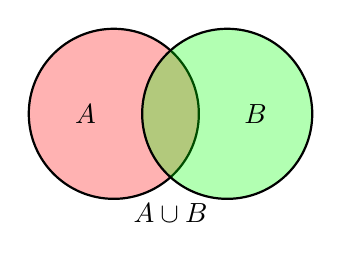
\begin{tikzpicture}[thick,fill opacity=0.3, every node/.style={opacity=1}, scale=.9]
\filldraw[fill=red] (0,0) circle (12mm);
\filldraw[fill=green] (16mm,0) circle (12mm);
\node at (-4mm,0) {$A$};
\node at (20mm,0) {$B$};
\node at (8mm,-14mm) {$A\cup B$};
\end{tikzpicture}%
}%
{%
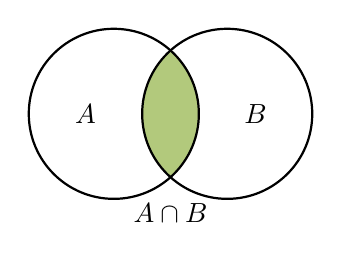
\begin{tikzpicture}[thick,fill opacity=0.3, every node/.style={opacity=1}, scale=.9]
\begin{scope}
\clip           (0,0) circle (12mm);
\clip             (16mm,0) circle (12mm);
\fill[fill=red] (0,0) circle (12mm);
\fill[fill=green] (16mm,0) circle (12mm);
\end{scope}
\draw           (0,0) circle (12mm);
\draw             (16mm,0) circle (12mm);
\node at (-4mm,0) {$A$};
\node at (20mm,0) {$B$};
\node at (8mm,-14mm) {$A\cap B$};
\end{tikzpicture}%
}%
{%
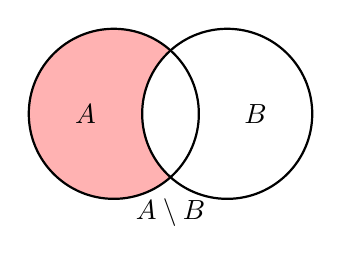
\begin{tikzpicture}[thick,fill opacity=0.3, every node/.style={opacity=1}, scale=.9]
\begin{scope}
\clip           (0,0) circle (12mm);
\fill[fill=red, even odd rule] (0,0) circle (12mm) (16mm,0) circle (12mm);
\end{scope}
\draw           (0,0) circle (12mm);
\draw             (16mm,0) circle (12mm);
\node at (-4mm,0) {$A$};
\node at (20mm,0) {$B$};
\node at (8mm,-14mm) {$A\setminus B$};
\end{tikzpicture}%
}%
{%
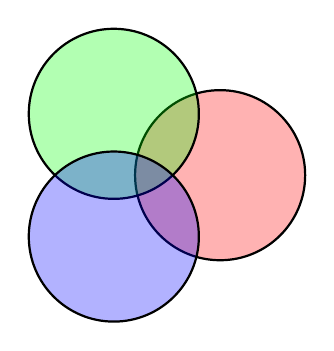
\begin{tikzpicture}[thick,fill opacity=0.3, every node/.style={opacity=1}, scale=.9]
\filldraw[fill=red] (0:1cm) circle (12mm);
\filldraw[fill=green] (120:1cm) circle (12mm);
\filldraw[fill=blue] (-120:1cm) circle (12mm);
\end{tikzpicture}\vspace*{-1cm}
}%
\задача
Сколько всего различных подмножеств в множестве из $n$ элементов?
\кзадача

%\УстановитьГраницы{0cm}{4cm}

\опр
\выд{Объединением\/} множеств $A$ и $B$ называют множество,
состоящее из всех таких~$x$, которые принадлежат хотя бы одному
из множеств $A$ или $B$ (т.~е. $x\in A$ или $x\in B$).
Обозначение:~\hbox{$A\cup B$}.\\
%\опр
\выд{Пересечением\/} множеств $A$ и $B$ называют множество,
состоящее из всех таких~$x$, что $x\in A$ и $x\in B$.
Обозначение:~$A\cap B$.\\
%\опр
\выд{Разностью\/} множеств $A$ и $B$ называют множество,
состоящее из всех таких~$x$, что $x\in A$ и $x\notin B$.
Обозначение:~$A\setminus B$.\\
Изображать объединение, пересечение и разность
удобно с помощью \выд{кругов Эйлера} (см. рис.)



\задача
Верно ли, что
\пункт $A\cup B = B \cup A$;
\пункт $A\cap B = B \cap A$;
\пункт $A\setminus B = B \setminus A$\,?
\кзадача

\задача
Пусть $A$~--- множество всех нечётных чисел,
$B$~--- множество всех чисел, делящихся на~3 ($A=\{2k+1 \mid k\in\Z\}$, $B=\{3k \mid k\in\Z\}$). Найдите $A\cap B$ и $B\setminus A$.
\кзадача

%\задача
%Для каждых двух из следующих множеств укажите их пересечение, объединение
%и разность: множество равнобедренных треугольников; множество треугольников
%с углом $110^\circ$; множество треугольников со стороной 7;
%множество треугольников, у которых наименьший угол равен $30^\circ$.

%\noindent
%{\small
%Чтобы доказать, что
%}

\задача
Верно ли, что для любых множеств $A$, $B$ и $C$\\
\вСтрочку
\пункт $A\setminus(A\setminus B) = A\cap B$;
\пункт $A\cap B = A \mbox{ тогда и только тогда, когда } A\subseteq B$; \\
\пункт $A\setminus B = C \mbox{ тогда и только тогда, когда } A=B\cup C$?
%\пункт $A\setminus(B\setminus C) = (A\setminus B)\cup(A\cap C)$.
\кзадача


\задача
Докажите тождества для любых множеств $A$, $B$ и $C$:\\
\вСтрочку
\пункт $A\cap(B\cap C) = (A\cap B)\cap C$;
\пункт $A\cup(B\cap C) = (A\cup B)\cap(A\cup C)$.
%\пункт $A\setminus(B\cap C) = (A\setminus B)\cup(A\setminus C)$.
\кзадача



\задача
\пункт В НИИ работают 67 человек. Из них
47 знают английский язык, 35 --- немецкий, и 23 --- оба языка.
Сколько человек в НИИ
не знают ни английского, ни немецкого языков?
\пункт Пусть кроме этого  польский
знают 20 человек, английский и польский --- 12, немецкий и
польский --- 11, все три языка --- 5.
Сколько человек не знают ни одного из этих языков?
\пункт [Формула включений и исключений]
Решите задачу в общем случае: имеется $m$ языков $L_1,\ L_2,\ldots,L_m$,
и для каждого набора языков $L_{i_1},\ L_{i_2},\ldots,L_{i_k}$ известно, что ровно $N_{i_1i_2\ldots i_k}$ человек знают все языки из этого набора.
\кзадача

\ВосстановитьГраницы


%\задача
%В ряд записали 105 единиц, поставив перед каждой знак \лк$+$\пк.
%Сначала изменили знак на противоположный перед каждой третьей единицей,
%затем --- перед каждой пятой, а затем --- перед
%каждой седьмой. Найдите значение полученного выражения.
%\кзадача


%\сзадача

%Какое максимальное количество различных множеств можно получить

%из данных~$n$, используя операции $\setminus$, $\cup$ и $\cap\,$?

%\кзадача

%\опр Для любого множества $A$ можно рассмотреть \выд{множество всех} его  {подмножеств}. Обозначение: $2^A$.
%\копр

\опр
\выд{Декартовым произведением} множеств $A$ и $B$ называется множество всевозможных упорядоченных пар $(a,b)$, где $a\in A$, $b \in B$. Обозначение: $A \times B = \{ (a,b) \mid a\in A, b\in B \}$.
\выд{Множество всех подмножеств} множества $A$ обозначается $2^A$.
\копр


\задача Пусть $\#A=m$, $\#B=n$. Найдите:
\вСтрочку
\пункт
$\#(A\times B)$;
\пункт
$\#2^A$.
\кзадача

%\задача
%На фикусе выросли 10 ананасов. Представьте множество способов сорвать несколько из них как декартово произведение нескольких множеств.
%\кзадача

\задача
Верно ли что
\вСтрочку
\пункт
$2^{A\times B} = 2^A \times 2^B$;
\пункт
$2^{A\cap B} = 2^A \cap 2^B$?
\кзадача

%\vfil


%\GenXMLW

\ЛичныйКондуит{0mm}{6mm}\vspace*{-4mm}

\end{document}


